ИУ7-55Б, 19\_BIS, Саблина\\
\let\oldclearpage\clearpage
\let\clearpage\relax


\chapter*{Введение}

\let\clearpage\oldclearpage

%Эффективное добавление деталей на изображения всегда было одной из основных проблем компьютерной графики \cite{procedural}. Процедурный шум является одним из наиболее успешных инструментов, используемых для создания таких деталей \cite{procedural}.

За последние 20 лет генерация текстур не перестала быть актуальной задачей компьютерной графики и упоминалась в \cite{procedural}\cite{focg}\cite{tandm}. Процедурный шум является одним из инструментов, используемых для решения данной задачи \cite{procedural}.
% Вариантом решения данной задачи является процедурный шум \cite{procedural}.

\textbf{Процедурным шумом} называют генерацию случайной и неструктурированной текстуры с помощью программного кода \cite{procedural}. Существует несколько видов реализаций процедурных шумов, одним из которых являются методы генерации шумов на решетке (lattice noises).

\textbf{Решеточные шумовые функции} генерируют шум путем интерполяции или свертки случайных значений и/или градиентов, определенных в точках целочисленной решетки \cite{procedural}. Типичным примером шума на решетке является шум Перлина \cite{procedural}.

%\chapter{Генерация шумов на решетке}
%\endgroup
%что значит генерация шумов на решётке

%Шум --- это случайный и неструктурированный паттерн, который полезен в случаях, когда необходим источник обширных деталей без явной структуры.

%...
%Процедурное текстурирование — метод создания текстур, при котором изображение текстуры создается с помощью какого-либо алгоритма (процедурного алгоритма). 
%[wiki]


%Методы генерации шумов на решетке являются наиболее популярными реализациями шума для приложений с процедурным текстурированием \cite{tandm}.



%\textbf{Целочисленной решеткой} называется набор всех точек в пространстве, координаты $x$, $y$ и $z$ которого имеют целочисленные значения \cite{perlin}\cite{tandm}.



% [State of the Art in Procedural Noise Functions]
%[Texturing and Modeling: A Procedural Approach (third edition) p. 69]

%the generation of a lattice noise begins with one or more uniformly distributed PRNs at every point in the texture space whose coordinates are integers. These points form the integer lattice. The necessary low-pass filtering of the noise is accomplished by a smooth interpolation between the PRNs. TO see why this works, recall that the correct reconstruction of a signal from a set of samples can never contain frequences higher than the Nyquist frequency of the same rate. Since the PRNs at the integer lattice points are equally spaced samples of white noise and since reconstruction from samples is a form of interpolation, it is reasonable to expect that the interpolated function will be approximately band-limited below the Nyquist frequency of the lattice interval. The quality of the resulting noise function depends on the nature of the interpolation scheme.
%All lattice noises need some way to generate one or more pseudorandom numbers at every lattice point.

%генерация решеточного шума начинается с одного или нескольких равномерно распределенных PRN в каждой точке текстурного пространства, координаты которой являются целыми числами. Эти точки образуют целочисленную решетку. Необходимая фильтрация нижних частот шума осуществляется путем плавной интерполяции между PRN. Чтобы понять, почему это работает, вспомните, что правильное восстановление сигнала из набора выборок никогда не может содержать частоты выше, чем частота Найквиста той же частоты. Поскольку PRN в целочисленных точках решетки представляют собой равноотстоящие отсчеты белого шума и поскольку реконструкция по выборкам является формой интерполяции, разумно ожидать, что интерполируемая функция будет приблизительно ограничена полосой пропускания ниже частоты Найквиста интервала решетки. Качество результирующей функции шума зависит от характера схемы интерполяции.
%Все шумы решетки требуют какого-то способа генерировать одно или несколько псевдослучайных чисел в каждой точке решетки.
%[Texturing and Modeling: A Procedural Approach (third edition) p. 69]

%\section{Градиентный шум}




%Lattice gradient noises generate noise by interpolating or convolving random values and/or gradients defined at the points of the integer lattice. The representative example of lattice gradient noises is Perlin noise.

\chapter{Шум Перлина}

%В 1985 году Кеном Перлином была представлена его известная шумовая функция. В [источник на статью перлина] данный метод описывается следующим образом:

%\begin{enumerate}
%	\item рассмотрим набор всех точек в пространстве, чьи координаты x, y и z имеют целочисленные значения. Мы называем это множество целочисленной решеткой.
	
%\end{enumerate}


В \cite{tandm}\cite{perlin}\cite{impperlin} метод генерации шума Перлина описан следующим образом:

%Шум определяется в точке пространства путем вычисления псевдослучайного градиента в каждой из восьми ближайших вершин целочисленной кубической решетки и выполнения интерполяции сплайнами.
\begin{enumerate}
	\item задать целочисленную решетку, то есть множество всех точек в пространстве, координаты которых являются целыми числами;
	%\item задаются массив $P$, содержащий псевдослучайную перестановку, и массив $G$, содержащий набор из 12 векторов, определяющих направления от центра куба до его ребер;
	\item задать массив $P$, содержащий псевдослучайную перестановку, и массив $G$, содержащий псевдослучайный набор градиентов единичной длины;
	\item с помощью хэш-функции $g = H(x, y, z)$, использующей массивы $P$ и $G$, связать с каждой точкой куба целочисленной решентки псевдослучайный градиент;
	 %целочисленной решетки псевдослучайный градиен; %псевдослучайное значение и координаты градиента: 
	%$[a,b,c,d] = H([x,y,z])$, где $[a,b,c,d]$ обозначает линейное уравнение градиента $[a,b,c]$ и значения $d$ в точке $[x, y, z]$;
	\item выполнить интерполяцию по трем направлениям восьми скалярных произведений $g_{i, j, k} \cdot (x - i, y - j, z - k)$, где $i, j, k$  --- координаты точек куба целочисленной решетки, а $g_{i, j, k}$ --- градиент в точке $(i, j, k)$.
	%\item если координаты точки находятся на целочисленной решетке, значение шумовой функции равно $d$, иначе вычислить значение шумовой функции с помощью интерполяции по трем направлениям.
\end{enumerate}

%Выровненные по координатам грани - это грани, которые имеют одинаковые значения координат на противоположных сторонах. Например, если у нас есть грань, выровненную по координате x, то значения координаты x будут одинаковыми на противоположных сторонах грани. То есть координаты точек на одной стороне грани будут иметь одинаковый x, в то время как координаты точек на противоположной стороне также будут иметь одинаковый x. Такое выравнивание координат может быть полезным при рассмотрении и обработке геометрических объектов.

В \cite{impperlin} уточняется, что в оригинальной версии алгорима генерации шума Перлина для интерполяции по трем направлениям была выбрана функция сглаживания
\begin{equation}
	\label{eq:old_s_func}
	s(t) = 3t^2 - 2t^3,
\end{equation}
где $t$ --- это значение координаты точки. Вторая производная функции (\ref{eq:old_s_func}) $6 - 12t$ не равна нулю при $t = 0$ и $t = 1$. Это ненулевое значение создает на выровненных по координатам гранях соседних кубических ячеек разрывы второго рода  \cite{impperlin}, влияние которых на внешний вид полученной текстуры отображено на рисунке \ref{fig:old_interpolant}.

Для решения этой проблемы функция (\ref{eq:old_s_func}) заменяется на
\begin{equation}
	\label{eq:new_s_func}
	6t^5 - 15t^4 + 10t^3,
\end{equation}
так как ее первая и вторая производные равны нулю при $t = 0$ и $t = 1$ \cite{impperlin}. На рисунке \ref{fig:new_interpolant} из \cite{impperlin} приведен результат замены функции сглаживания.

\clearpage
\begin{figure}[h]
	\centering
	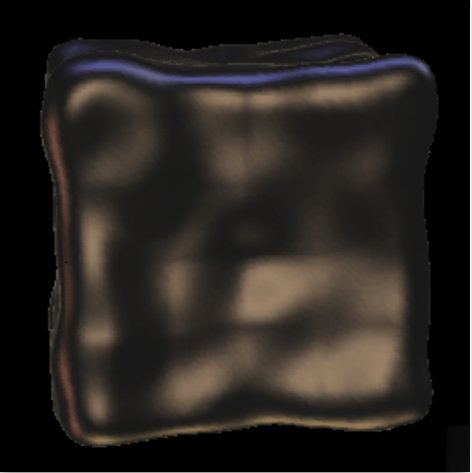
\includegraphics[height=0.3\textheight]{img/old_interpolant.pdf}
	\caption{Шум Перлина, полученный с использованием функции сглаживания (\ref{eq:old_s_func}), рисунок Кена Перлина \cite{impperlin}}
	\label{fig:old_interpolant}
\end{figure}

\begin{figure}[h]
	\centering
	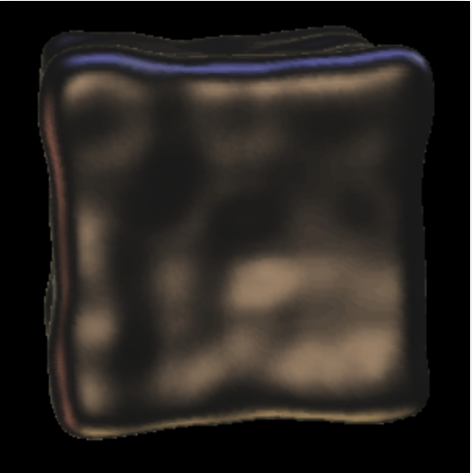
\includegraphics[height=0.3\textheight]{img/new_interpolant.pdf}
	\caption{Шум Перлина, полученный с использованием функции сглаживания (\ref{eq:new_s_func}), рисунок Кена Перлина \cite{impperlin}}
	\label{fig:new_interpolant}
\end{figure}
\clearpage

Следующей проблемой, описанной в \cite{impperlin}, является то, что в массиве $G$ содержатся градиенты единичной длины, но в кубической решетке расстояния от центра куба до его ребер укорочены вдоль осей и удлинены вдоль диагоналей между противоположными углами куба. Это приводит к тому, что близлежащие градиенты сливаются друг с другом, из-за чего шумовая функция принимает аномально высокие значения в этих областях \cite{impperlin}, что отображено на рисунке \ref{fig:old_g} из \cite{impperlin}. 

Для решения данной проблемы массив $G$ заменяют набором из 12 векторов, определяющих направления от центра куба до его ребер. Чтобы избежать затрат на деление на 12, Перлином предложено увеличить набор до 16 градиентов, добавляя в него дополнительные $(1,1,0)$, $(-1,1,0)$, $(0,-1,1)$ и $(0,-1,-1)$ \cite{impperlin}. На рисунке \ref{fig:new_g} из \cite{impperlin} приведен результат замены массива градиентов $G$.

\clearpage
\begin{figure}[h]
	\centering
	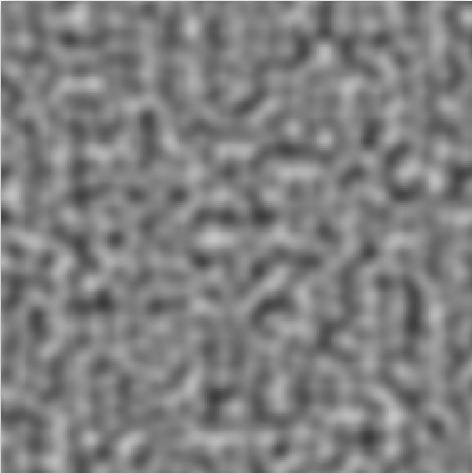
\includegraphics[height=0.3\textheight]{img/old_g.pdf}
	\caption{Шум Перлина, полученный с использованием старого массива градиентов $G$, рисунок Кена Перлина \cite{impperlin}}
	\label{fig:old_g}
\end{figure}

\begin{figure}[h]
	\centering
	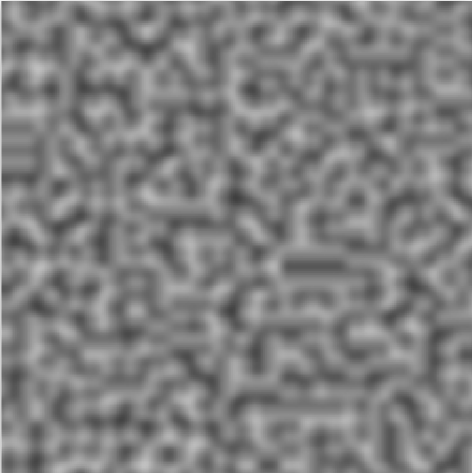
\includegraphics[height=0.3\textheight]{img/new_g.pdf}
	\caption{Шум Перлина, полученный с использованием нового массива градиентов $G$, рисунок Кена Перлина \cite{impperlin}}
	\label{fig:new_g}
\end{figure}





%Пусть $(i, j, k)$ обозначают восем точек куба, где $i$ --- это набор нижних и верхних ограничивающих целых чисел $x: \{|x|, |x| + 1\}$ и, аналогично, $j = \{|y|, |y| + 1\}$ и $k = \{|z|, |z| + 1\}$. Восемь градиентов задаются формулой $\mathbf{g_{i,j,k}} = G[P[P[P[i] + j] + k]]$, где $P$ является предварительно вычисленным массивом, содержащим  псевдослучайную перестановку, а $G$ --- набором из 12 векторов, определяющих направления от центра куба до его ребер:

%\begin{center}
%$(1,1,0),(-1,1,0),(1,-1,0),(-1,-1,0),$\\
%$(1,0,1),(-1,0,1),(1,0,-1),(-1,0,-1),$\\
%$(0,1,1),(0,-1,1),(0,1,-1),(0,-1,-1)$\\
%\end{center}

%Последовательное применение $P$ хэширует каждую точку решетки и градиенты из описанного набора выбираются использованием результата $P$ по модулю 12. Чтобы избежать затрат на деление на 12, предлагается увеличить набор до 16 градиентов, добавляя в него дополнительные $(1,1,0)$, $(-1,1,0)$, $(0,-1,1)$ и $(0,-1,-1)$.

%Восемь скалярных произведений $\mathbf{g_{i,j,k} \cdot (x - i, y - j, z - k)}$ затем подвергаются интерполяции по трем направлениям. Для интерполяции используются измененные координаты точек $s(x - |x|)$, $s(y - |y|)$ и $s(z - |z|)$, где
%\begin{equation}
%	\label{eq:s1}
%	s(t) = 6t^5 - 15t^4 + 10t^3.
%\end{equation}




%\subsection{Better Gradient Noise}

%В \cite{bettergrad} авторы предлагают 3 улучшения градиентного шума Перлина:

%\begin{enumerate}[label=---]
%\item В оригинальном алгоритме генерации шума Перлина для любых значений $(i, j, k)$, которые хэшируются как $P[0]$, соседняя точка решетки $(i, j, k + 1)$ хэшируется как $P[1]$. Таким образом, каждый столбец будет выдавать одинаковые сдвинутые последовательности значений. Чтобы исправить этот недостаток, предлагается использовать отдельные таблицы перестановок для каждого направления $P_x$, $P_y$, $P_z$ и искать индекс градиента в таблице $G$, используя исключающее ИЛИ, $P_x[i] \oplus P_y[j] \oplus P_z[k]$.
%\item Функция (\ref{eq:s1}) заменяется на
%\begin{equation}
%	\label{eq:s2}
%s(t) = (2 − t)^4(2 + t)^4(1 − t)(1 + t)/256 = 4(1 − t^2/4)^5 − 3(1 − t^2/4)^4.
%\end{equation}
%Данная модификация улучшает ограничение диапазона получаемых значений \cite{procedural}.
%\item Также предложен метод проекции полученного шума на плоскость.
%\end{enumerate}

%В \cite{bettergrad} приведены результаты улучшения шума Перлина (рисунок \ref{img:better_gradient_noise}).
%\clearpage

%\begin{figure}[h]
%	\centering
%	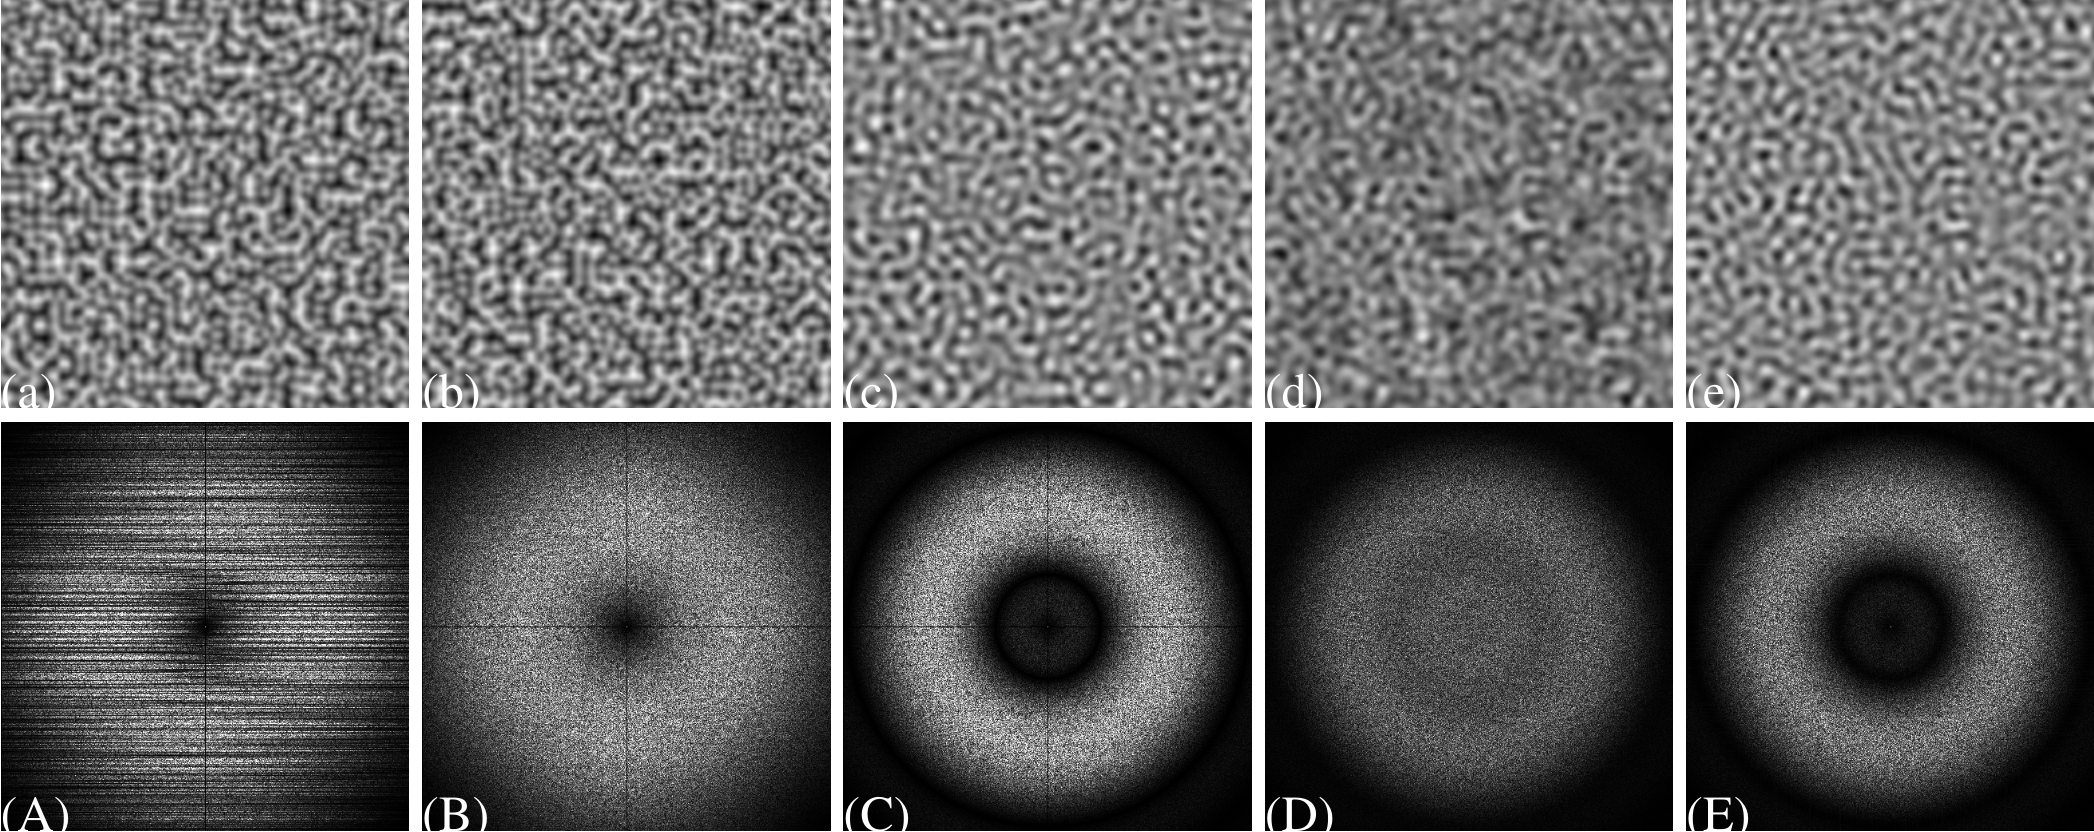
\includegraphics[width=0.9\textwidth]{img/better_gradient_noise.png}
%	\caption{Better Gradient Noise}
%	\label{img:better_gradient_noise}
%\end{figure}



%На рисунке \ref{img:better_gradient_noise} изображены:
%\begin{enumerate}[label=---]
%	\item (a) 2D шум Перлина без модификаций;
%	\item (b) 2D шум Перлина с хэш-функцией, использующей исключающее ИЛИ;
%	\item (c) 2D шум с измененной функцией $s(t)$;
%	\item (d) <<разрез>> модифицированного 3D шума на плоскости;
%	\item (e) 2D шум, полученный с помощью метода проекции на плоскость.
%\end{enumerate}


